\section{Background}
\label{sec:background}

\begin{figure}[t!]
\centering
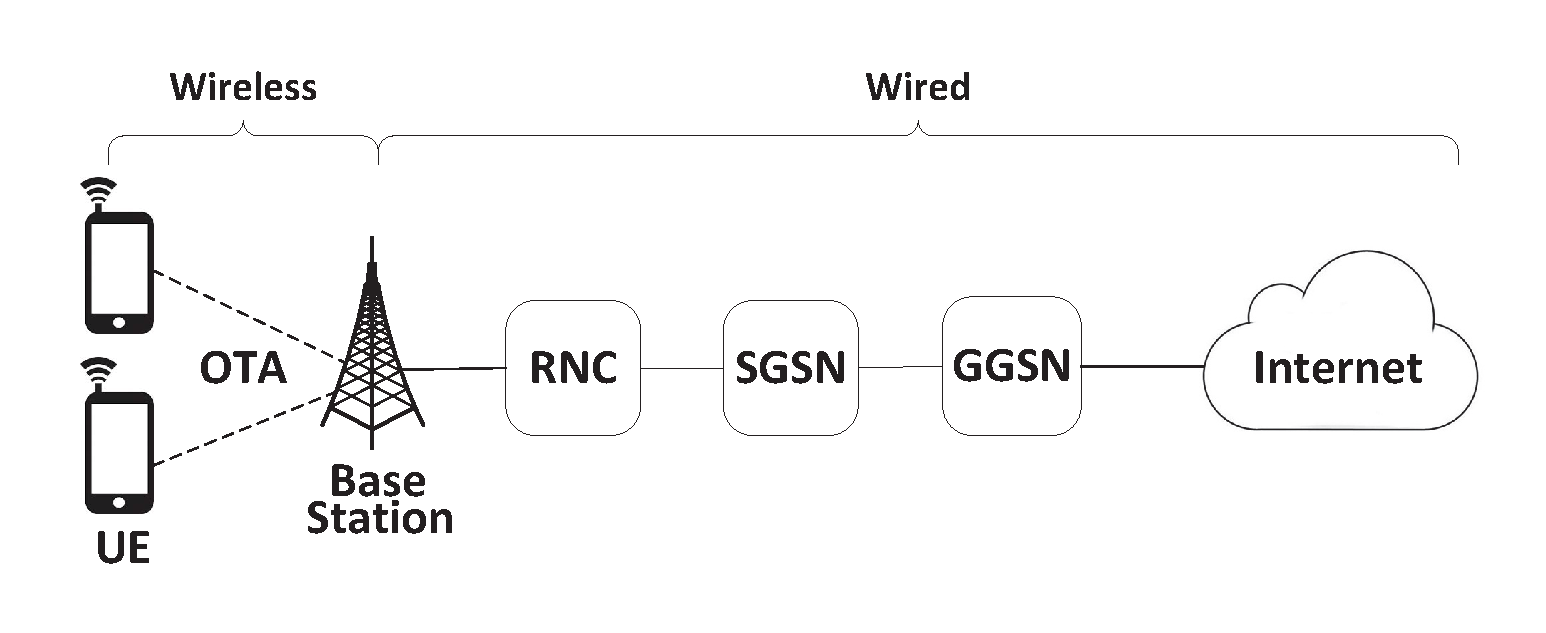
\includegraphics[width=0.5\textwidth]{figs/cellular_network_topology.eps}
\caption{The general cellular network architecture}
\label{fig:cell.topology}
\end{figure}

As illustrated in Figure~\ref{fig:cell.topology}, in both 3G UMTS~\cite{3gpp.3G} and 4G LTE networks~\cite{3gpp.LTE}, data is transmitted from \textit{user equipment} (UE), i.e. mobile devices,  to the base station (Node B in UMTS, eNB in LTE), then to the \textit{Serving GPRS support node} (SGSN) and \textit{Gateway GPRS support node} (GGSN), and ultimately to the server~\cite{umts_book}. The link between the UE and the base station is known as the \textit{over-the-air} (OTA) link, and it is the only wireless link in the network topology. The rest of the links from the base station to the internet are all wired.

\subsection{Radio Resource Control} 
\label{subsec:background.rrc}
\begin{figure}[t!]
\centering
\includegraphics[width=0.5\textwidth]{figs/RRC_State_Diagram.pdf}
\caption{Possible 3G and 4G State Machines as Specified by 3GPP.} 
\label{fig:statemachine}
\end{figure}

Mobile cellular networks use the RRC protocol as the control plane signaling for Layer 3 to allocate resources to mobile devices.  Handsets transition between different RRC states, which vary in power consumption and bandwidth, and an individual RRC state machine is maintained for each handset.  Transitions between different states occur due to traffic patterns between the device and base station. In general, more traffic will cause a higher-power and higher-bandwidth state to be entered.  The RRC protocol for these network types has been defined by 3GPP~\cite{spec-3G-RRC, spec-LTE-RRC}.

For 3G UMTS~\cite{spec-3G-RRC}, there are three main states:  DCH, which is high-power and high-bandwidth, FACH, which is low power and low bandwidth, and PCH, where no transmission is possible. If a higher-bandwidth state is needed, there is a promotion delay. Some carriers may always go directly from PCH to DCH. An example RRC state machine can be seen at the top of Figure~\ref{fig:statemachine}.

For 4G~\cite{spec-LTE-RRC}, the state machine is more complicated, and is summarized in the bottom half of Figure~\ref{fig:statemachine}.  We are concerned mainly with transitions between RRC\_{}CONNECTED, a higher-power state, and RRC\_{}IDLE, a lower-power state where no data is transmitted. The other states have timers on the orders of tens or hundreds of milliseconds are are not practical to measure on end-user devices, as tools such as a power monitor are required.

\subsection{Radio Link Control}

\begin{figure}[t!]
\centering
\includegraphics[width=0.5\textwidth]{figs/RLC_group_ack.eps}
\caption{RLC PDU transmission in Acknowledged Mode. When the sender sends out a polling request, the receiver will respond with a "group" of acknowledge in terms of the starting PDU sequence number and the consecutive PDU loss length.}
\label{fig:rlc.protocol}
\end{figure}

RLC protocol is a packet fragmentation protocol that used as the data plane transmission for cellular air interface~\cite{spec-3G-RLC}. There are three different modes that configured by the upper layer: TM (Transparent Mode), UM (Unacknowledged Mode), and AM (Acknowledged Mode). RLC in TM directly pass the packet from PDCP (Packet Data Convergence Protocol) layer to MAC layer, and it usually applies for voice transmission. RLC in UM sends the PDU (Packet Data Unit), which is smallest data fragmentation unit, without waiting for any response from the receiver (in this case, Node B or eNB). RLC usually transmit VoIP traffic with UM. RLC in AM deploys an ARQ (Automatic Repeat reQuest) mechanism. As show in Figure~\ref{fig:rlc.protocol}, RLC sender periodically piggybacks the polling request in the RLC header, and the receiver will respond with a RLC STATUS PDU which contains groups of not received PDU sequence numbers. We call this particular ARQ mechanism as \textit{group acknowledgement}. Since RLC transmit both TCP and UDP with AM, we will assume the rest of RLC transmission mechanism to be AM.
\label{subsec:background.rlc}